\documentclass[a4paper,12pt]{article}

\usepackage[margin=1.15in]{geometry}
\usepackage[utf8]{inputenc}
\usepackage[T1]{fontenc}
\usepackage{fancyhdr}
\usepackage{listings}
\usepackage{graphicx}
\usepackage{ragged2e}
\usepackage{tabularx}
\usepackage{amsmath}
\usepackage{systeme}
\usepackage{float}
\usepackage{color}
\usepackage{alltt}

\def\arraystretch{1.25}
\usepackage{listings}
\usepackage[dvipsnames]{xcolor}
\usepackage[portuguese]{babel}

\lstset{
language=Octave,
backgroundcolor=\color{white},   % choose the background color; you must add \usepackage{color} or \usepackage{xcolor}
basicstyle=\footnotesize\ttfamily,        % the size of the fonts that are used for the code
breakatwhitespace=false,         % sets if automatic breaks should only happen at whitespace
breaklines=true,                 % sets automatic line breaking
captionpos=b,                    % sets the caption-position to bottom
commentstyle=\color{gray},    % comment style
%escapeinside={\%*}{*)},          % if you want to add LaTeX within your code
extendedchars=true,            % lets you use non-ASCII characters; for 8-bits encodings only, does not work with UTF-8
frame=single,                    % adds a frame around the code
% frameround=fttt,
keepspaces=true,                 % keeps spaces in text, useful for keeping indentation of code (possibly needs columns=flexible)
classoffset=0,
keywordstyle=\color{RoyalBlue},       % keyword style
deletekeywords={function,endfunction, if,endif},
classoffset=1,
morekeywords={function,endfunction, if,endif},
keywordstyle=\bf\color{Red},       % keyword style
classoffset=2,
morekeywords={persistent},            % if you want to add more keywords to the set
keywordstyle=\bf\color{ForestGreen},       % keyword style
classoffset=0,
literate=
{/}{{{\color{Mahogany}/}}}1
{*}{{{\color{Mahogany}*}}}1
{.*}{{{\color{Mahogany}.*}}}2
{+}{{{\color{Mahogany}+{}}}}1
{=}{{{\bf\color{Mahogany}=}}}1
{-}{{{\color{Mahogany}-}}}1
{[}{{{\bf\color{RedOrange}[}}}1
{]}{{{\bf\color{RedOrange}]}}}1
{ç}{{\c{c}}}1 % Cedilha
{á}{{\'{a}}}1 % Acentos agudos
{é}{{\'{e}}}1
{í}{{\'{i}}}1
{ó}{{\'{o}}}1
{ú}{{\'{u}}}1
{â}{{\^{a}}}1 % Acentos circunflexos
{ê}{{\^{e}}}1
{î}{{\^{i}}}1
{ô}{{\^{o}}}1
{û}{{\^{u}}}1
{à}{{\`{a}}}1 % Acentos graves
{è}{{\`{e}}}1
{ì}{{\`{i}}}1
{ò}{{\`{o}}}1
{ù}{{\`{u}}}1
{ã}{{\~{a}}}1 % Tils
{ẽ}{{\~{e}}}1
{ĩ}{{\~{i}}}1
{õ}{{\~{o}}}1
{ũ}{{\~{u}}}1,
numbers=left,                    % where to put the line-numbers; possible values are (none, left, right)
numbersep=6pt,                   % how far the line-numbers are from the code
numberstyle=\tiny\color{gray}, % the style that is used for the line-numbers
rulecolor=\color{black},         % if not set, the frame-color may be changed on line-breaks within not-black text (e.g. comments (green here))
showspaces=false,                % show spaces everywhere adding particular underscores; it overrides 'showstringspaces'
showstringspaces=false,          % underline spaces within strings only
showtabs=false,                  % show tabs within strings adding particular underscores
stepnumber=1,                    % the step between two line-numbers. If it's 1, each line will be numbered
stringstyle=\color{purple},     % string literal style
tabsize=2,                       % sets default tabsize to 2 spaces
title=\lstname,                   % show the filename of files included with \lstinputlisting; also try caption instead of title
}

\title{\Huge \textbf{Numerical Methods} \\
       \vspace{+0.3cm} \LARGE Ex. 10. Approximate Solving of Ordinary Differential Equations.}

\author{Kamila Kwiecińska, Karol Latos}

\date{
\centering
\begin{tabularx}{\textwidth} {| >{\centering\arraybackslash}X |}
 \hline
 Group \textbf{2}, team \textbf{2}, 22.05.2020 \\
 \hline
\end{tabularx}}

\begin{document}

\maketitle

\justifying

\section{Introduction}
Differential equations are the mathematical backbone of myriad of useful models not only in physics, chemistry and biology, but also in economics, social sciences and more. However, solving them is not always a straightforward task; moreover, in the age of computers, numerical methods are needed for acquiring solutions to differential-type problems. Some of these methods were implemented in Octave language in order to solve following differential equations:

\begin{equation}
\label{ODE}
    y^{(1)}(x) = -5.8y(x) + 4.7x - 0.9x^{2},\quad y(x_{0} = 0) = 1.9,\quad 0\leq x \leq 9.
\end{equation}

\begin{equation}
\label{SODE}
\begin{split}
y^{(2)}(x) + 2y^{(1)}(x) = 30\cos(x),\quad y(&x_{0} = 0) = 8, \\
&y^{(1)}(x_{0} = 0) = 11,\quad 0 \leq x \leq 10.
\end{split}
\end{equation}


\subsection{Requirements for the report}
\begin{enumerate}
    \item Solve Equation (\ref{ODE}) using Taylor series method. Restrict the solution to three terms of the Taylor series. Present this solution on a graph. Discuss the results.
    \item Use your program for Euler method to solve Equation (\ref{ODE}) numerically. Present the obtained solutions in the form of a single graph for integration steps \linebreak[4] $h \in \{0.01, 0.1, 1.0\}$. Discuss the results.
    \item Use your program for fourth order Runge-Kutta method to solve Equation (\ref{ODE}) numerically. Present the obtained solutions in the form of a single graph for integration steps $h \in \{0.01, 0.1, 1.0\}$. Discuss the results.
    \item Explain the differences between the solutions obtained in 1., 2. and 3.
    \item Use your program for fourth order Runge-Kutta method to solve Equation (\ref{SODE}) numerically. Present the obtained solutions in the form of a single graph for integration steps $h \in \{0.01, 0.1, 1.0\}$. Discuss the results. Plot a separate graph, that will present the relation between $y_i$ (X axis) and $y^{(1)}_i$ (Y axis), for each integration step h value.
    \item Estimate, discuss, and compare errors of each numerical method you implemented.
    \item Write down your observations and conclusions from the exercise.
    \item Include all source codes.
\end{enumerate}

\section{Solving Equation (\ref{ODE}) using three methods}

\subsection{Taylor series method}
To obtain three terms of the Taylor series for $y(x)$, two additional derivatives ought to be calculated:
\begin{align*}
    &y^{(2)}(x) = -5.8y^{(1)}(x) + 4.7 - 1.8x \\
    &y^{(3)}(x) = -5.8y^{(2)}(x) - 1.8
\end{align*}

From abbreviated Taylor expansion it holds that
\begin{equation}
    \label{taylor}
    y(x) \approx y(x_0) + y^{(1)}(x_0)(x-x_0) + \frac{y^{(2)}(x_0)}{2}(x-x_0)^2 + \frac{y^{(3)}(x_0)}{6}(x-x_0)^3,
\end{equation}

using $x_0 = 0$ from the initial condition and substituting consecutive values gives
\begin{align*}
    &y(x_0) = 1.9,
    &y^{(1)}(x_0) = -11.02, \\
    &y^{(2)}(x_0) = 68.616,
    &y^{(3)}(x_0) = -399.7728.
\end{align*}

Now equation (\ref{taylor}) is used to finally obtain
\begin{equation}
    y(x) \approx -66.6288x^3 + 34.308x^2 - 11.02x + 1.9
\end{equation}

It is nothing unusual for Taylor series polynomials approximating non-polynomial functions to quickly diverge from the approximated function, especially when the number of terms is low. That's why we see values around negative 45000 at $x = 9$ (Fig. \ref{fig:taylor_big}). Taking a closer look at the interval near $x_0$, one can observe closeness to the approximated function (Fig. \ref{fig:taylor_small}). One cannot help but wonder, what was the purpose of that exercise in relation to the report, except for proving that the student can calculate simple derivatives and plug the number 0 as argument of functions.

\begin{figure}[H]
    \centering
    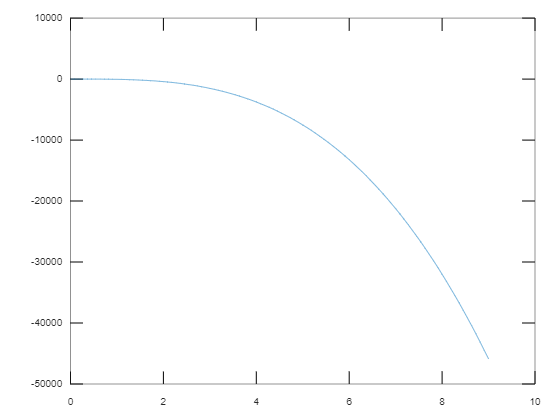
\includegraphics[width=0.9\textwidth]{taylor_big.png}
    \caption{Taylor series polynomial approximating $y$}
    \label{fig:taylor_big}
\end{figure}
\begin{figure}[H]
    \centering
    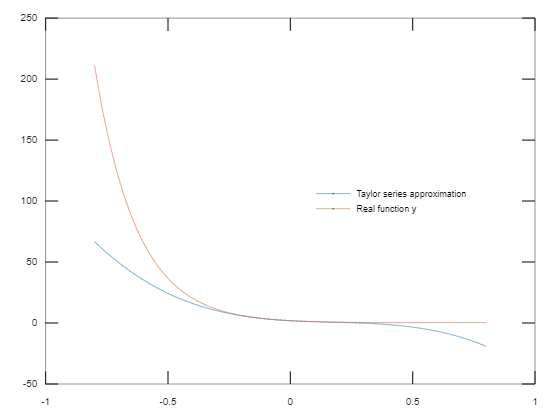
\includegraphics[width=0.9\textwidth]{taylor_small.png}
    \caption{Taylor series polynomial approximating $y$ - interval around $x_0$}
    \label{fig:taylor_small}
\end{figure}

\subsection{Euler-Cauchy method}
Following graphs show the approximation of $y$ function being a solution to Equation (\ref{ODE}). Additional graph without step $h = 1$ has been included, as step values above 0.7 yield unexpected results with very high values, rising in an exponential fashion.

\begin{figure}[htp]
    \centering
    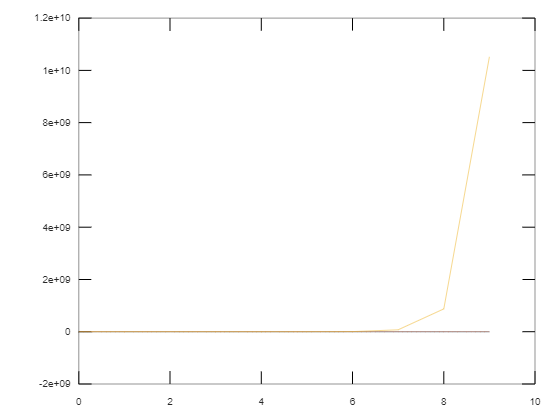
\includegraphics[width=\textwidth]{euler_cauchy_all.png}
    \caption{Euler-Cauchy method with h $= 0.01, 0.1$ and $1$}
    \label{fig:euler_cauchy_all}
\end{figure}
\begin{figure}[htp]
    \centering
    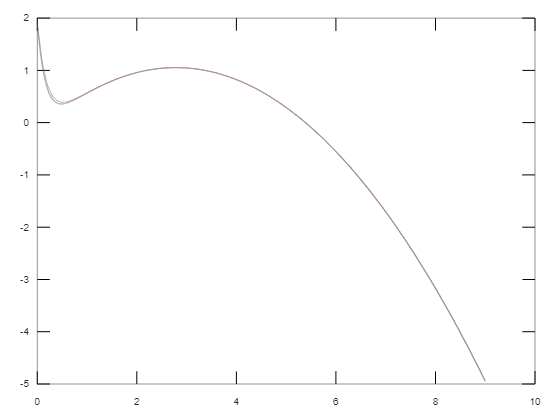
\includegraphics[width=0.9\textwidth]{euler_cauchy_two.png}
    \caption{Euler-Cauchy method with h $= 0.01$ and $0.1$}
    \label{fig:euler_cauchy_two}
\end{figure}

It can be seen that, despite some little difference around the local minimum, there is not much discrepancy between step 0.1 and 0.01, as both approximate the $y$ function closely (Fig. \ref{fig:euler_cauchy_two}).

\subsection{Runge-Kutta method}
Following graphs show the approximation of $y$ function being a solution to Equation (\ref{ODE}). Additional graph without step $h = 1$ has been included, again, as step values above 0.7 yield unexpected results.

\begin{figure}[H]
    \centering
    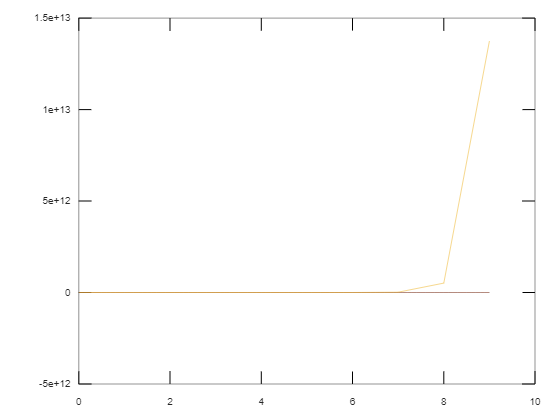
\includegraphics[width=\textwidth]{runge_kutta_all.png}
    \caption{Runge-Kutta method with $h = 0.01, 0.1$ and $1$}
    \label{fig:runge_kutta_all}
\end{figure}
\begin{figure}[H]
    \centering
    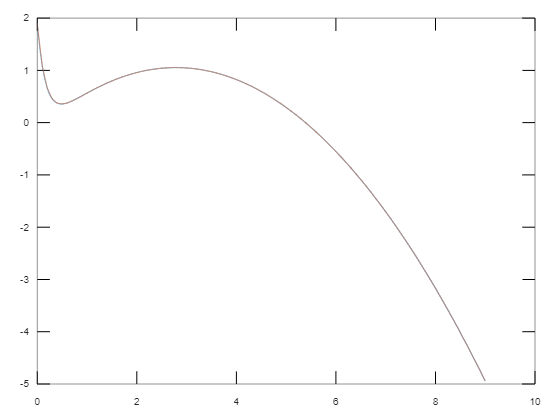
\includegraphics[width=\textwidth]{runge_kutta_two.png}
    \caption{Runge-Kutta method with $h = 0.01$ and $0.1$}
    \label{fig:runge_kutta_two}
\end{figure}

It can be seen, again, that there is not much difference between step 0.1 and 0.01, as both approximate the $y$ function closely.

\subsection{Results commentary}

Both Euler-Cauchy and Runge-Kutta methods were easy to implement and are not very resource- nor time-consuming. At first glance the noticeable differences between these two methods restrict themselves to the number of lines of code used in the main iteration loop (3 and 6, respectively) and the slight separation of approximation curves in Euler-Cauchy, which may signify lower accuracy. Thus, the reader is advised to try both methods on their own, as so far most of the conclusions concerning the differences between the methods has appeared as feelings and therefore cannot be easily transcribed.

\section{Solving Equation (\ref{SODE}) using Runge-Kutta method}
The second order differential equation (\ref{SODE}) can be rewritten as presented:
\begin{equation}
    y^{(2)}(x) = -2y^{(1)}(x) + 30\cos(x)
\end{equation}
\clearpage
Using a simple substitution, a system of first order differential equations is obtained.

\begin{gather}
    \begin{cases}
    y^{(1)}(x) = z(x) \\ z^{(1)}(x) = -2y^{(1)}(x) + 30\cos(x)
    \end{cases}
\end{gather}

Solving this system using fourth order Runge-Kutta method yields promising results, with better and better approximation of the $y$ function, as $h$ gets smaller and smaller (Fig \ref{fig:runge_kutta_sode}).

\begin{figure}[H]
    \centering
    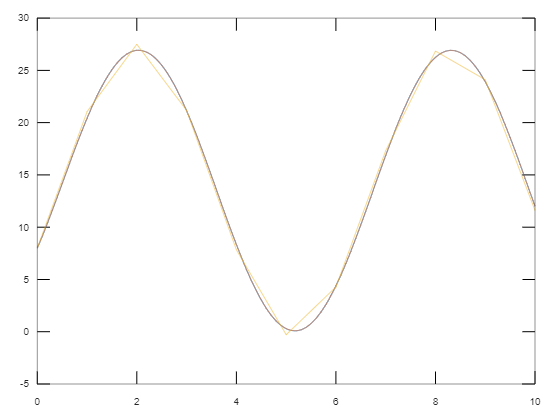
\includegraphics[width=0.7\textwidth]{runge_kutta_sode.png}
    \caption{Runge-Kutta method for Eq. (\ref{SODE}) with $h = 0.01, 0.1$ and $1$}
    \label{fig:runge_kutta_sode}
\end{figure}

\begin{figure}[H]
    \centering
    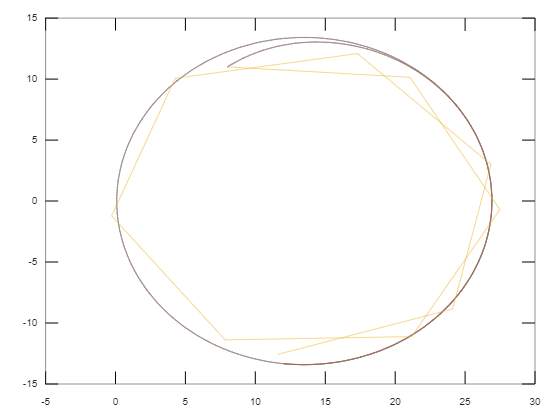
\includegraphics[width=0.7\textwidth]{yz.png}
    \caption{Relationship between $y$ (X axis) and $y^{(1)}$ (Y axis)}
    \label{fig:yz}
\end{figure}

\section{Errors analysis}
The error after $n$ iterations of Euler method can be bound from above by $Mh\frac{e^{Lhn} - 1}{2L}$. To perform more useful analysis, original $y$ function is calculated:

\begin{equation}
    y(x) = -0.155169x^2 + 0.86383x - 0.14893 + \frac{2.04893}{e^{5.8x}}
\end{equation}

Now, for each approximating function $A$, new function is created according to the pattern. 

\begin{equation}
    m(A, y) = | A(x) - y(x) |
\end{equation}

Using any numerical integration method, the differences between the approximating and approximated functions are summed up.

\begin{equation}
    M(A, y) = \int_{x_0}^{x_n} m(A, y) dx
\end{equation}

Therefore, $M(A, y)$ returns the total space in between $A$ and $y$ on $[x_0, x_n]$ interval. It's worth noting, that
\begin{gather*}
    \lim_{A \to y} M(A, y) = 0 \iff \lim_{M(A, y) \to 0} A = y.
\end{gather*}

Comparing Euler-Cauchy and Runge-Kutta methods with this approach, with $0.01 \leq h \leq 0.3$, yields results visible in Fig \ref{fig:error_1}. Since Euler-Cauchy method is unstable (the error is propagated with each iteration), there is no point in considering $h > 0.3$, as the values of errors rise, rendering the Runge-Kutta method errors insignificant.

\begin{figure}[H]
    \centering
    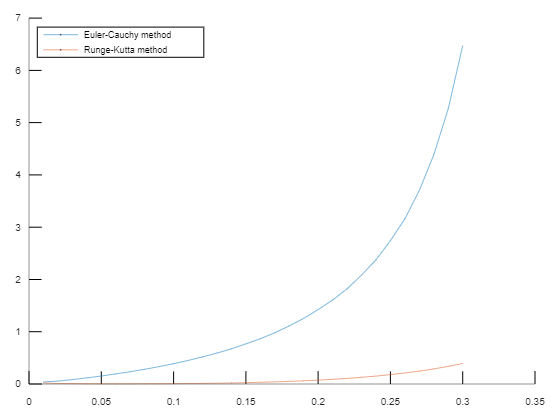
\includegraphics[width=0.9\textwidth]{error_1.png}
    \caption{$M(A, y)$ (error) values for E-C and R-K methods}
    \label{fig:error_1}
\end{figure}

Similarly, $y$ function being a solution to Equation (\ref{SODE}) is firstly calculated:
\begin{equation}
    y(x) = \frac{1}{2}\left(e^{-2x} + 24\sin(x) - 12\cos(x) + 27\right)
\end{equation}

Applying function $M$ for approximations of $y$ in relation to the integration step $h \in \left[0.01, 1\right]$, gives the following error graph.

\begin{figure}[H]
    \centering
    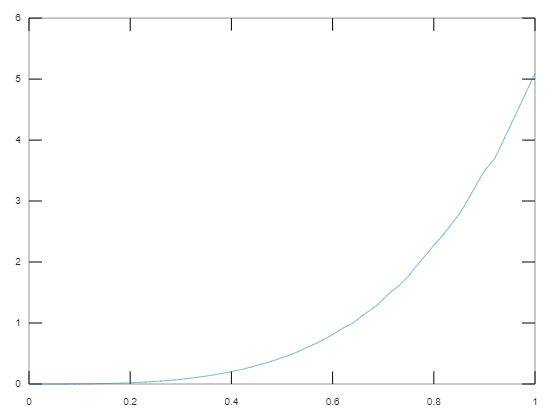
\includegraphics[width=0.8\textwidth]{error_2.png}
    \caption{$M(A, y)$ (error) value R-K method in Eq. (\ref{SODE})}
    \label{fig:error_2}
\end{figure}

The Runge-Kutta method rises far more slowly than Euler-Cauchy, even when used for solving second order differential equations through substitution. The error near $h = 0$ is as little, as it is near $h = 0.2$, which signifies great accuracy. 

\section{Conclusions}
Implementation of selected methods for solving ordinary differential equations was easy and pleasurable. No obstacles were faced and the approaches resulted in successful approximation of the $y$ functions. The Euler-Cauchy method was the simplest, requiring the least amount of memory, time and lines of code --- however, as an unstable method, the error was being propagated through every iteration. This characteristic could be observed in the comparison between the errors of two methods: Euler-Cauchy and Runge-Kutta, in section 4. The latter alogrithm was found to be superior. As comes to solving second order differential equations, the Runge-Kutta method was more than suitable, and combined with converting the equation into a system of first order differential equations, yielded approximations of great accuracy, as could be concluded from error analysis. The exercise, as it is stated in subsection 1.1 and performed in this report, is recommended to anyone in need for a good fun combined with a bit of education.

\section{Code}
\lstset{language=Octave}
\begin{lstlisting}
# Karol Latos & Kamila Kwiecinska
value = 0.0;

# Coefficients for equations
global a_1 = -5.8;
global b_1 = 4.7;
global c_1 = -0.9;
global d_1 = 1.9;
global e_1 = 9;
global a_2 = 2;
global b_2 = 30;
global c_2 = 8;
global d_2 = 11;
global e_2 = 10;

# Function f, right-hand side of the ODE
function value = f(x, y)
    global a_1 b_1 c_1;
    value = a_1 * y + b_1 * x + c_1 * x^2;
end

# Initial condition as a point satifying y(x_0) = y_0
x_0 = 0;
y_0 = d_1;

# Integration step
h = 0.1;

# Euler-Cauchy method
M = [x_0, y_0];
for i = 1:e_1/h
    M(i + 1, 1) = M(i, 1) + h;
    y_rough = M(i, 2) + h * f(M(i, 1), M(i, 2));
    M(i + 1, 2) = M(i, 2) + 0.5 * h * (f(M(i, 1), M(i, 2)) + f(M(i + 1, 1), y_rough));
end

printf("Euler-Cauchy method\nStep h = %d\n", h);
printf("Obtained points:\n");
disp(M)
figure(1);
plot(M(:, 1), M(:, 2))

# Runge-Kutta method
M = [x_0, y_0];
for i = 1:e_1/h
    k_1 = h * f(M(i, 1), M(i, 2));
    k_2 = h * f(M(i, 1) + 0.5 * h, M(i, 2) + 0.5 * k_1);
    k_3 = h * f(M(i, 1) + 0.5 * h, M(i, 2) + 0.5 * k_2);
    k_4 = h * f(M(i, 1) + h, M(i, 2) + k_3);
    M(i + 1, 1) = M(i, 1) + h;
    M(i + 1, 2) = M(i,2) + (k_1 + 2*k_2 + 2*k_3 + k_4)/6;
end

printf("\nRunge-Kutta method\nStep h = %d\n", h);
printf("Obtained points:\n");
disp(M)
figure(2);
plot(M(:, 1), M(:, 2))

# y^(2) = -a_2 * y^(1) + b_2 * cos(x) /\ y^(1) = z(x)
# z^(1) = -a_2 * z(x) + b_2 * cos(x)
function value = f1(x, y, z)
    global a_2 b_2;
    value = -a_2 * z + b_2 * cos(x);
end

function value = f2(x, y, z)
    value = z;
end

# Initial condition points
x_0 = 0;
y_0 = c_2;
y_1 = d_2;

x = x_0:h:e_2;
y = zeros(size(x)(2), 1);
z = zeros(size(x)(2), 1);
y(1) = y_0;
z(1) = y_1;

k_1 = zeros(4, 1);
k_2 = zeros(4, 1);
for i=2:1:size(x)(2)
    k_1(1) = h*f2(x(i-1), y(i-1), z(i-1));
    k_2(1) = h*f1(x(i-1), y(i-1), z(i-1));
    k_1(2) = h*f2(x(i-1) + h/2, y(i-1) + k_1(1)/2, z(i-1) + k_2(1)/2);
    k_2(2) = h*f1(x(i-1) + h/2, y(i-1) + k_1(1)/2, z(i-1) + k_2(1)/2);
    k_1(3) = h*f2(x(i-1) + h/2, y(i-1) + k_1(2)/2, z(i-1) + k_2(2)/2);
    k_2(3) = h*f1(x(i-1) + h/2, y(i-1) + k_1(2)/2, z(i-1) + k_2(2)/2);
    k_1(4) = h*f2(x(i-1) + h, y(i-1) + k_1(3), z(i-1) + k_2(3));
    k_2(4) = h*f1(x(i-1) + h, y(i-1) + k_1(3), z(i-1) + k_2(3));
    y(i) = y(i-1) + (k_1(1) + 2*k_1(2) + 2*k_1(3) + k_1(4))/6;
    z(i) = z(i-1) + (k_2(1) + 2*k_2(2) + 2*k_2(3) + k_2(4))/6;
end
M = [x', y];

printf("\nRunge-Kutta method for 2nd order\nStep h = %d\n", h);
printf("Obtained points:\n");
disp(M)
figure(3);
plot(x, y);
\end{lstlisting}
\end{document}